%%%%%%%%%%%%%%%%%%%%%%%%%%%%%%%%%%%%%%
%%%%%%%%%%%%%%%%%%%%%%%%%%%%%%%%%%%%%%
% Do not edit the TeX file your work
% will be overwritten.  Edit the RnW
% file instead.
%%%%%%%%%%%%%%%%%%%%%%%%%%%%%%%%%%%%%%
%%%%%%%%%%%%%%%%%%%%%%%%%%%%%%%%%%%%%%





\newcommand{\DefineMacros}{
\newcommand{\SimNumObs}{5,000}
\newcommand{\SimTrueTheta}{0.5}
\newcommand{\SimAccNumObs}{5,000}
\newcommand{\SimAccSigx}{2}
\newcommand{\SimAccSigeps}{1}
\newcommand{\SimAccPercentMax}{10}
\newcommand{\MxNoise}{757.8}
\newcommand{\MxBetahat}{-4.55}
\newcommand{\MxNobs}{16,560}

}

%%%%%%%%%%%%%%%%%%%%%%
%%%%%%%%%%%%%%%%%%%%%%
%%%%%%%%%%%%%%%%%%%%%%
% Tables

\newcommand{\CashTransfersResultsTable}{
% \input{figures/cash_transfers_re_run_table.tex}


\begin{table}\small 
\begin{tabular}{|ccc|}
\toprule
 Original estimate (SE) & Refit estimate (SE)  & Observations dropped \\
\midrule
\midrule
33.861 (4.468)* &  -9.416 (3.296)* &  986 = 9.37\%\\
\midrule
\bottomrule
\end{tabular}
\caption{ Cash transfers results (N = 10518) \citep{angelucci2009indirect} }
\label{table:cash_transfers_re_run_table}
\end{table}


}

%%%%%%%%%%%%%%%%%%%
% OHIE

\newcommand{\OHIEResultsTable}{
% \input{figures/OHIE_table_9_IV_re_run_table.tex}


\begin{table}\small 
\begin{tabular}{|ccc|}
\toprule
 Original estimate (SE) & Refit estimate (SE)  & Observations dropped \\
\midrule
\midrule
0.029 (0.005)* &  -0.009 (0.004)* &  224 = 0.96\%\\
\midrule
\bottomrule
\end{tabular}
\caption{ Medicaid profit results (N = 23361) \citep{finkelstein2012oregon} }
\label{table:ohie_profit_results_reg}
\end{table}


}


%%%%%%%%%%%%%%%%%%%
% Microcredit
%
\newcommand{\MicrocreditProfitResultsTable}{
% \input{figures/microcredit_profit_re_run_table.tex}


\begin{table}\small 
\begin{tabular}{|ccc|}
\toprule
 Original estimate (SE) & Refit estimate (SE)  & Observations dropped \\
\midrule
\midrule
-4.549 (5.879) &  7.030 (2.549)* &  15 = 0.09\%\\
\midrule
\bottomrule
\end{tabular}
\caption{ Microcredit Mexico results (N = 16560) \citep{angelucci2015microcredit}. }
\label{table:mc_profit_results}
\end{table}


}
%
%
% \newcommand{\MicrocreditTemptationResultsTable}{
% % \input{figures/microcredit_profit_re_run_table.tex}
% <<microcredit_temptation_results_table, cache=microcredit_cache, results='asis'>>=
% source("figures_knitr/microcredit/microcredit_temptation_results_table.R",
%        echo=knitr_debug, print.eval=TRUE)
% @
% }

%%%%%%%%%%%%%%%%%%%
% Microcredit mixture
%
% \newcommand{\MicrocreditMixtureResultsTable}{
% <<mcmix_re_run_table, cache=mcmix_cache, results='asis'>>=
% source("figures_knitr/microcredit_mixture/microcredit_mix_refit_table.R",
%        echo=knitr_debug, print.eval=TRUE)
% @
% }
%
% \newcommand{\MicrocreditMixtureSdResultsTable}{
% <<mcmix_sd_re_run_table, cache=mcmix_cache, results='asis'>>=
% source("figures_knitr/microcredit_mixture/microcredit_mix_sd_refit_table.R",
%        echo=knitr_debug, print.eval=TRUE)
% @
% }

%%%%%%%%%%%%%%%%%%%%%%
%%%%%%%%%%%%%%%%%%%%%%
%%%%%%%%%%%%%%%%%%%%%%
% Graphs


\newcommand{\SimInflHistogram}{

\begin{knitrout}
\definecolor{shadecolor}{rgb}{0.969, 0.969, 0.969}\color{fgcolor}

{\centering 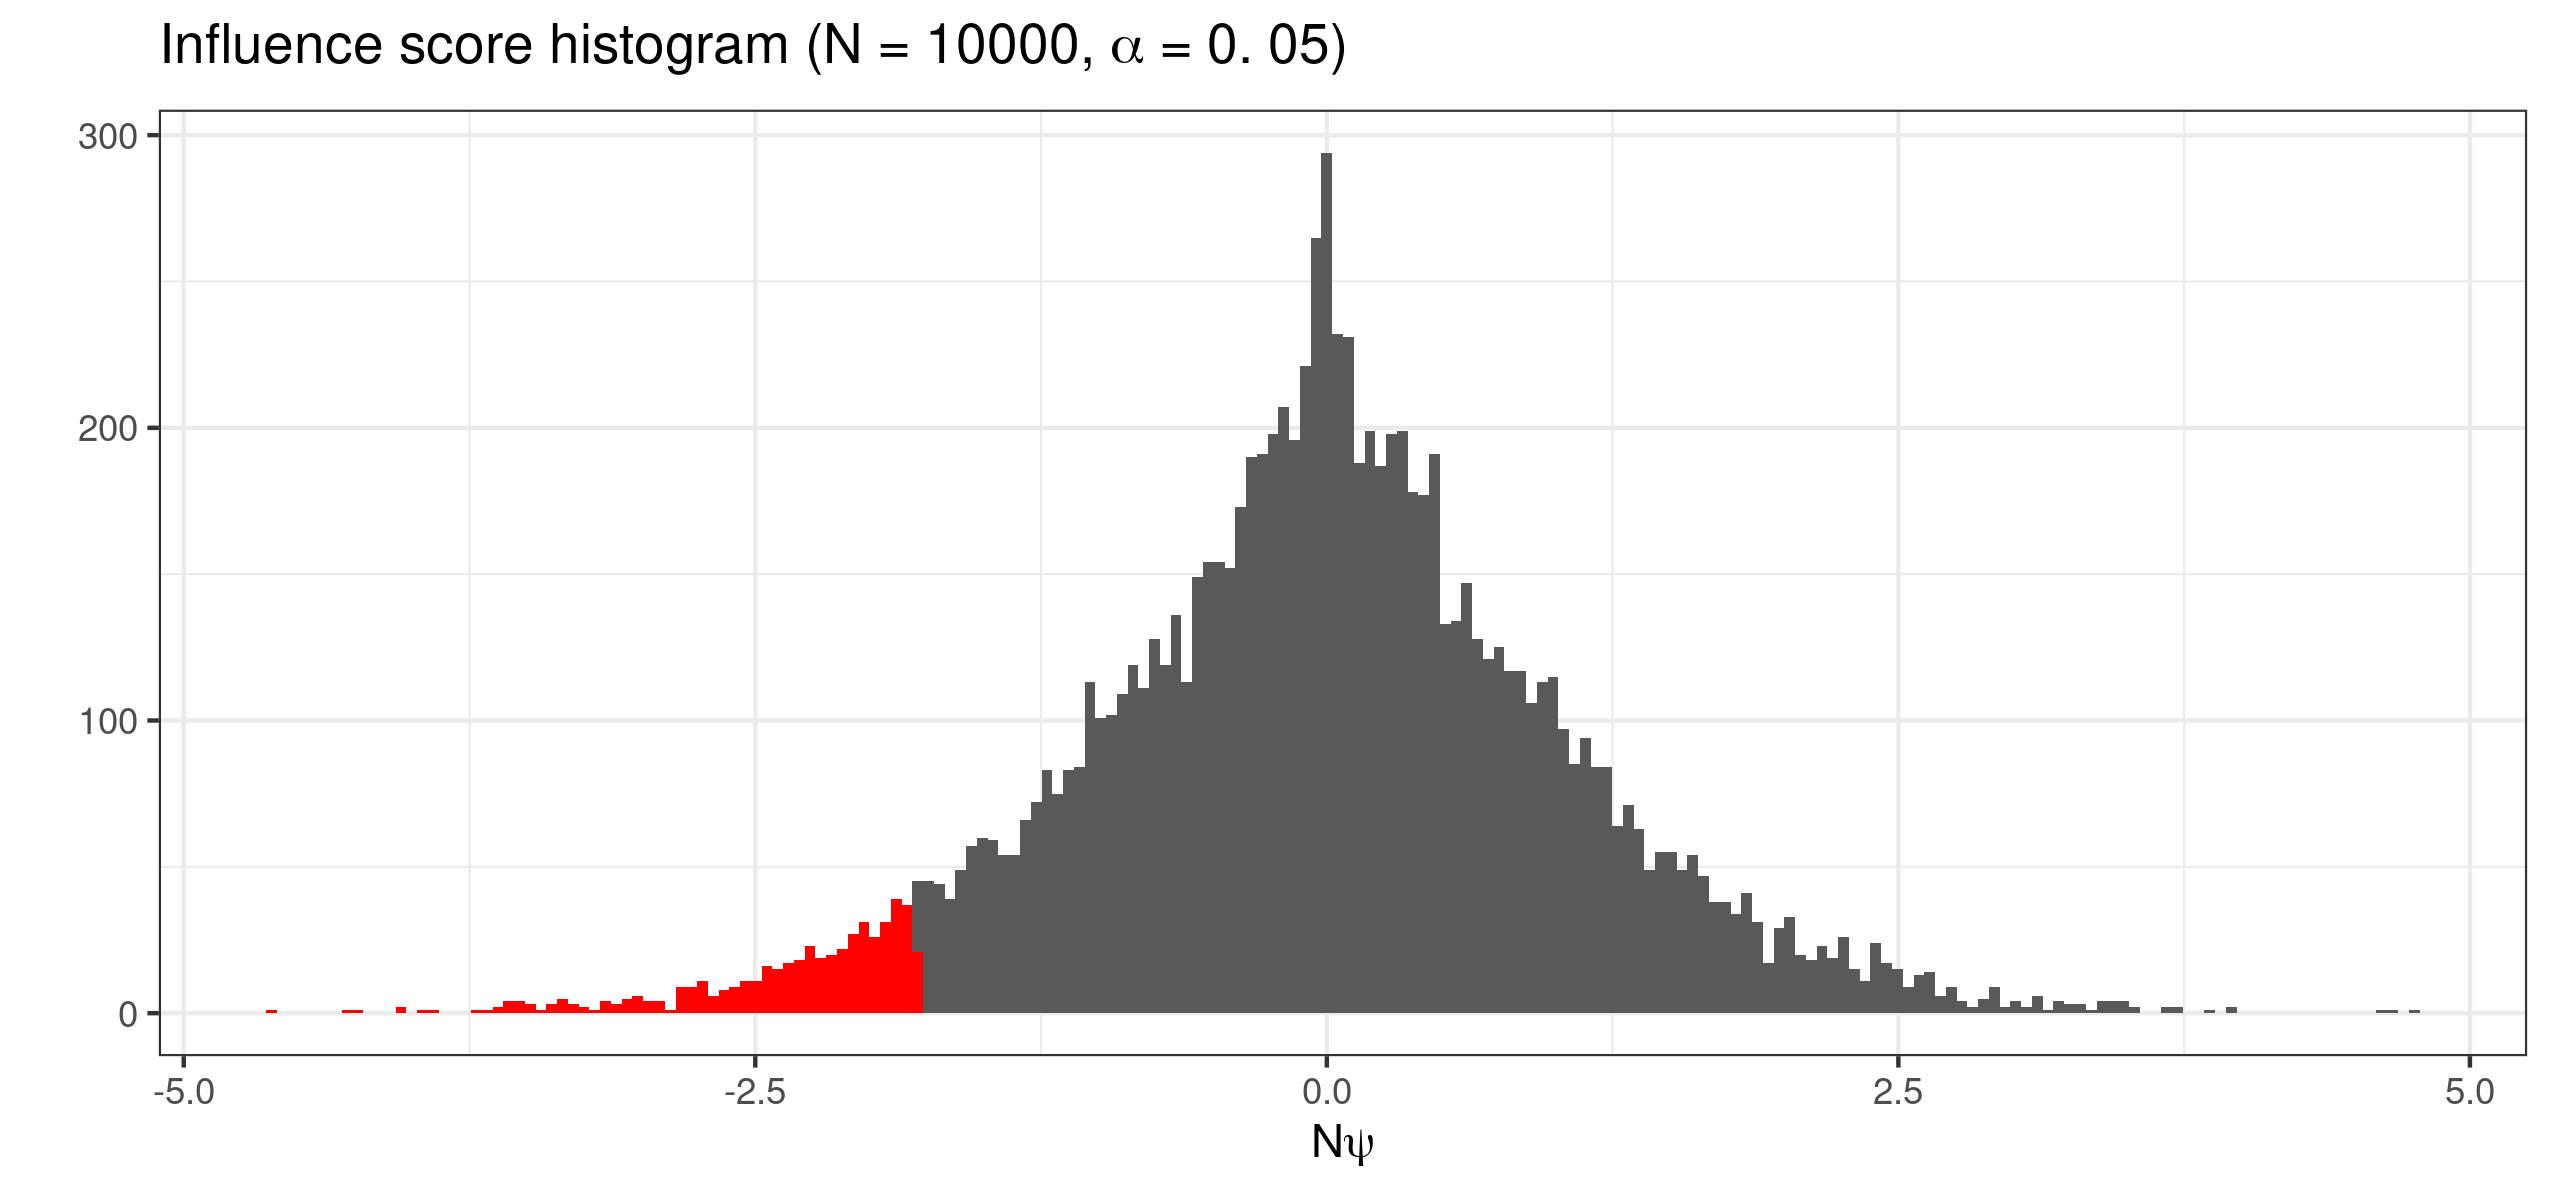
\includegraphics[width=0.98\linewidth,height=0.461\linewidth]{figure/sim-infl-hist-1} 

}



\end{knitrout}
}





\newcommand{\SimRefitOne}{
\begin{knitrout}
\definecolor{shadecolor}{rgb}{0.969, 0.969, 0.969}\color{fgcolor}

{\centering 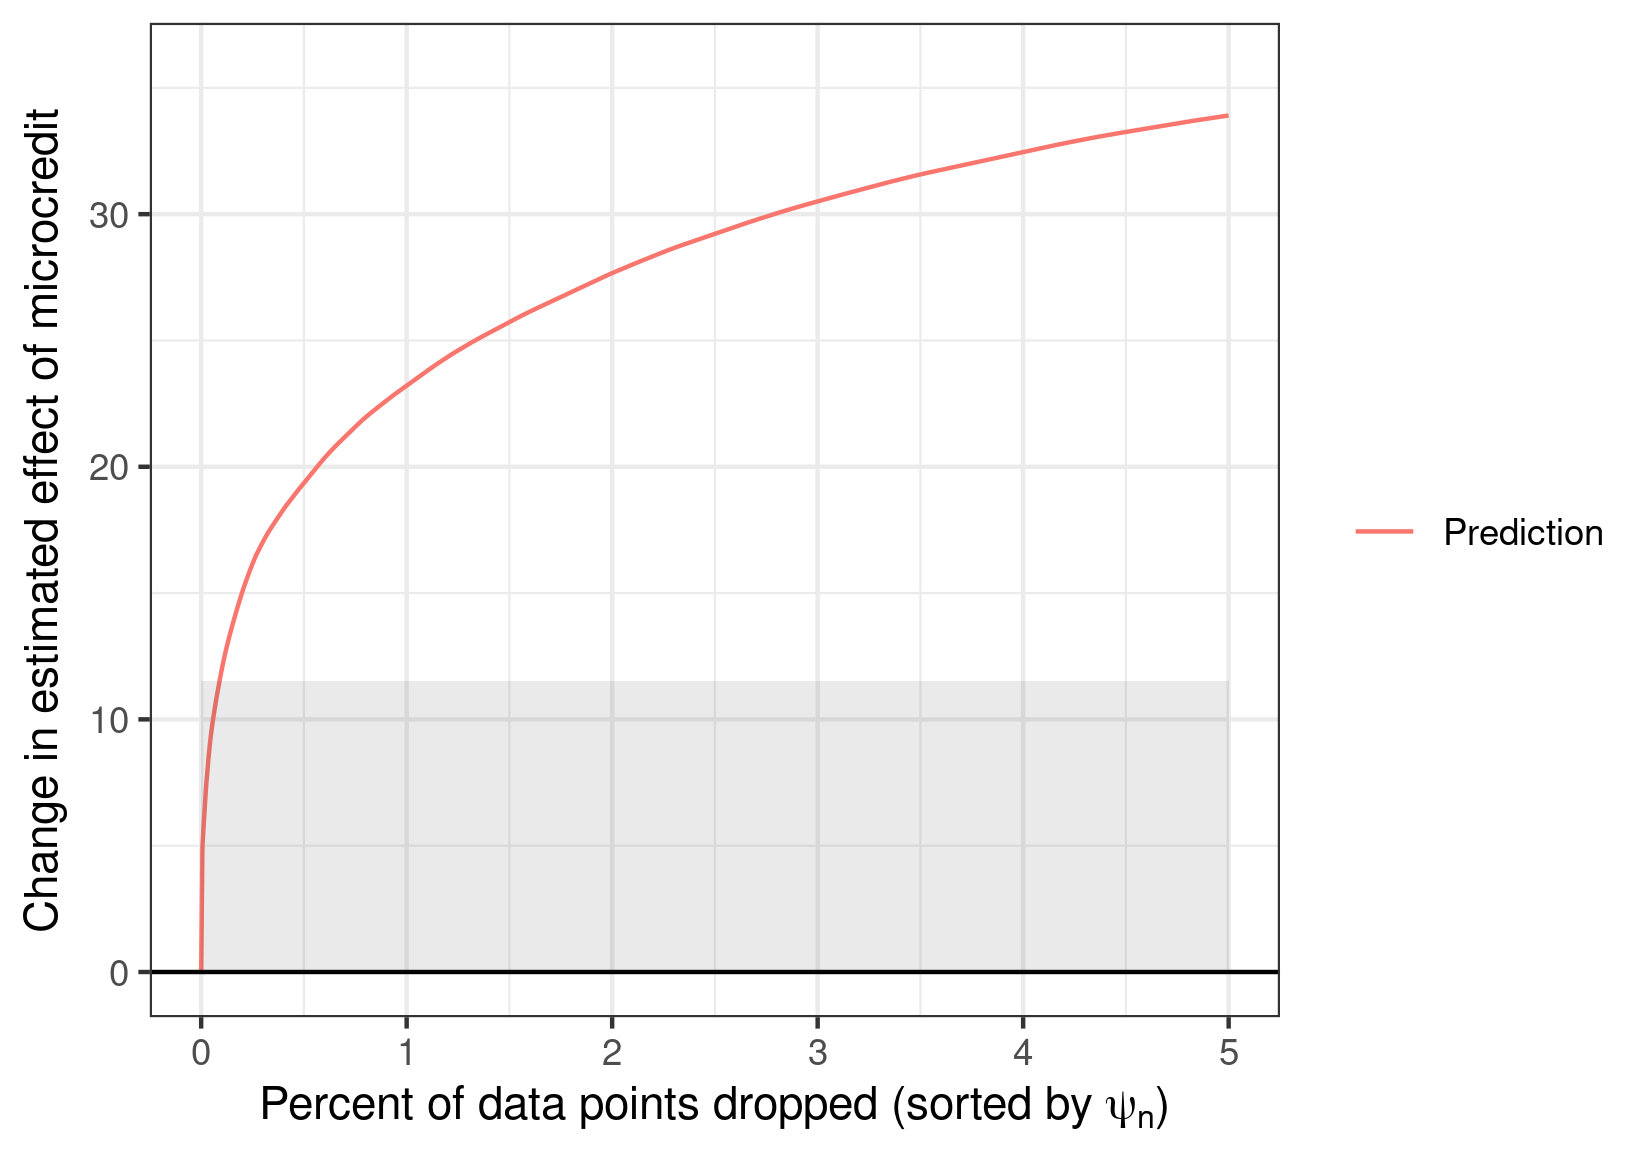
\includegraphics[width=0.98\linewidth,height=0.692\linewidth]{figure/sim-refit-one-1} 

}



\end{knitrout}
}

\newcommand{\SimRefitTwo}{
\begin{knitrout}
\definecolor{shadecolor}{rgb}{0.969, 0.969, 0.969}\color{fgcolor}

{\centering 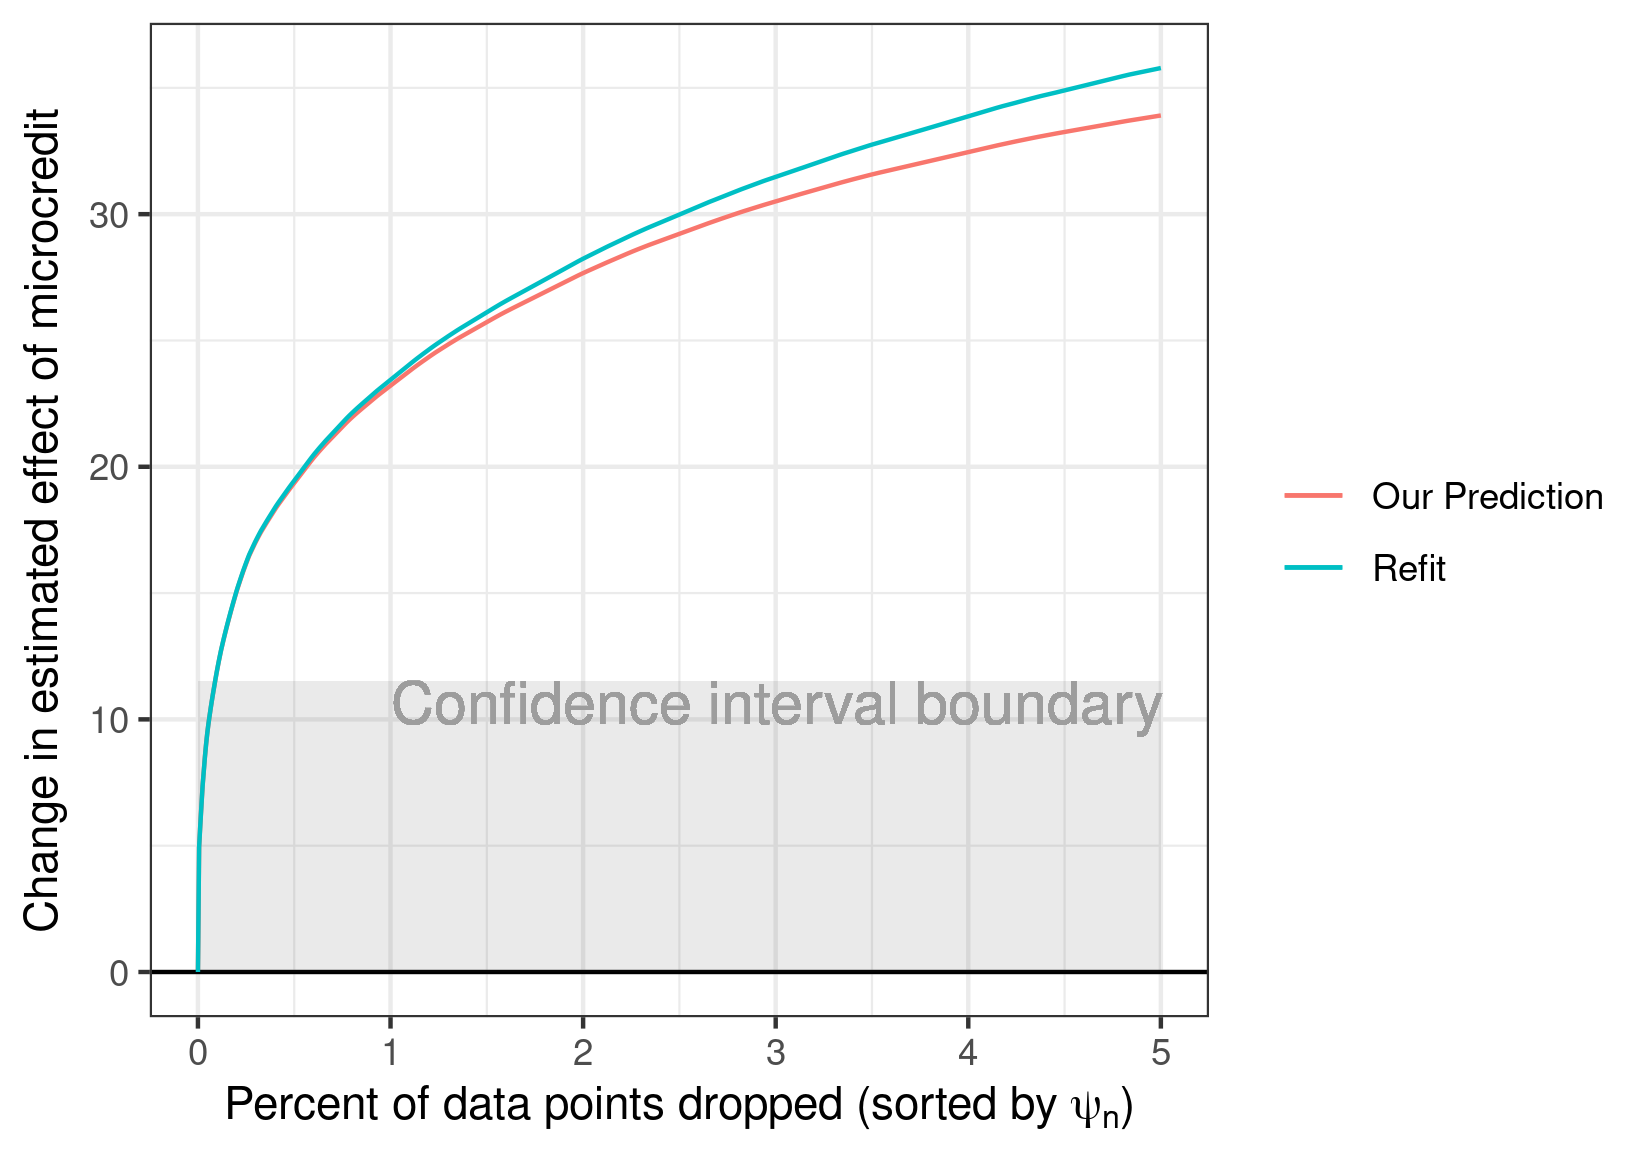
\includegraphics[width=0.98\linewidth,height=0.692\linewidth]{figure/sim-refit-two-1} 

}



\end{knitrout}
}



% \newcommand{\SimApproxNormalGraph}{
% <<sim_graphics_cap4>>=
% figcap <- paste0(
%     "The actual change, linear approximation to the change, ",
%     "and approximation error.",
%     "Here, $\\sigma_x = \\SimAccSigx$, ",
%     "$\\sigma_\\varepsilon = \\SimAccSigeps$, and ",
%     "$\\theta_0 = \\SimTrueTheta$.")
% SetImageSize(aspect_ratio=base_aspect_ratio / 1.5)
% @
% <<sim-approx-normal, cache=sim_cache, fig.show='hold', fig.cap=figcap>>=
% source("figures_knitr/simulations/graphs_comb.R",
%        echo=knitr_debug, print.eval=TRUE)
% print(plot2)
% SetFullImageSize()
% @
% }
%
% \newcommand{\SimGridNormalGraph}{
% <<sim_graphics_cap5>>=
% figcap <- paste0(
%     "The approximate perturbation inducing proportion ",
%     "at differing values of $\\sigma_x$ ",
%     "and $\\sigma_\\varepsilon$. Red colors indicate datasets whose sign can ",
%     "is predicted to change when dropping less than 1\\% of datapoints. ",
%     "The grey areas indicate ",
%     "$\\amip{\\alpha} = \\na$, a failure of the linear approximation to ",
%     "locate any way to change the sign.")
% SetImageSize(aspect_ratio=base_aspect_ratio / 1.8)
% @
% <<sim-grid-normal, cache=sim_cache, fig.show='hold', fig.cap=figcap>>=
% source("figures_knitr/simulations/graphs_comb.R",
%        echo=knitr_debug, print.eval=TRUE)
% print(plot1)
% SetFullImageSize()
% @
% }
